\section{Sprint 1}
Lors du premier sprint, nous avons dû mettre en place la base du programme.\\ Pour le modèle, il s'agissait de mettre en place les classes :
\begin{itemize}
\item Turtle qui représente une tortue, 
\item Point, pour stocker les coordonnées d'une tortue,
\item Line, qui permettent aux tortues de laisser une trace (instruction pendown),
\item World.\\
\end{itemize}
Voir l'UML~\ref{v0.1} correspondant page~\pageref{v0.1}.\\
\begin{figure}[h]
\caption{\label{v0.1} UML de la version 0.1 prévue}
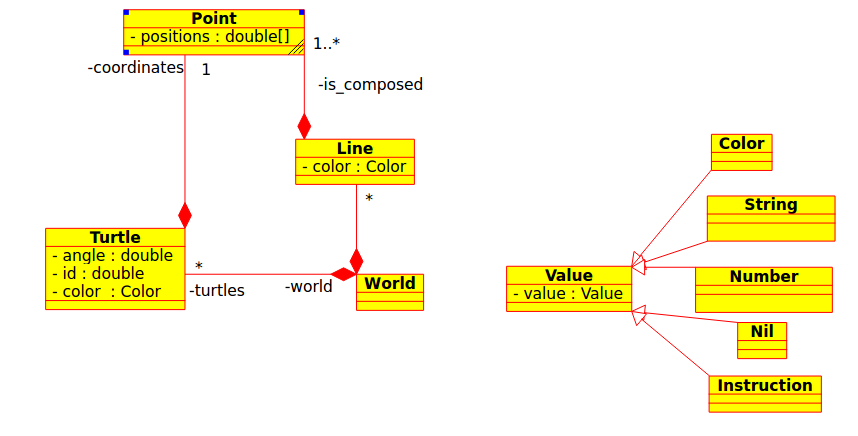
\includegraphics[scale=0.5]{doc/report/uml/v01.png}
\end{figure}
\newpage
La classe World représente le monde des tortues. Il contient la liste des tortues, et les lignes tracées par ces tortues.
Nous mettons aussi en place certains types Stibbons, comme Color, pour la couleur, ou Nil qui a une valeur nulle. Ils héritent de Value, une classe abstraite qui contient une valeur et ses accesseurs.\\

A la fin du premier sprint, nous avions réalisé ce schéma, en dehors de la classe Instruction qui n'était pas nécessaire. Les instructions tel que pendown, forward, etc... sont finalement des mots clés dans la grammaire du langage.\\
Voir figure~\ref{v0.1R} page~\pageref{v0.1R}.
\begin{figure}[h]
\caption{\label{v0.1R} UML de la version 0.1 réalisée}
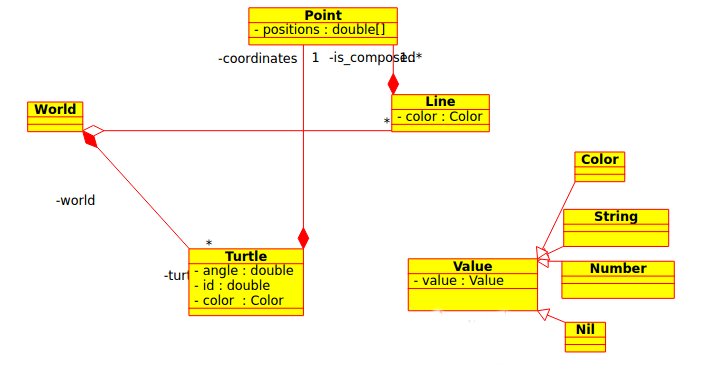
\includegraphics[scale=0.5]{doc/report/uml/v01reel.png}
\end{figure}
CAPTURE D'ECRAN DE L'APPLI

\section{Sprint 2}
Pour le second sprint, nous avons ajouté une classe Agent, car les classes World, Turtle et Zone sont des agents, au sens multi-agent.\\ Ils ont chacun un parent, celui qui l'a créer, une liste d'enfant, et des propriétés. Les propriétés sont des variables définit par l'utilisateur lors de la définition du code de l'agent, donc surtout utile pour les tortues.\\
Le monde a une taille, une liste de "breed", d'espèce. Il y a les espèces nommées et les "anonymes", qui sont des turtles dans le code.\\
Comme le montre ce code, on peut créer des tortues nommées ou pas.\\
METTRE UN EXEMPLE DE CODE DE L'UTILISATION DE BREED\\

Les types stibbons sont les mêmes, mais leurs définitions s'est un peu compléxifier en passant par une classe Simple-value, pour la mise en place des mutexs. Une énumeration des types Stibbons existe, elle est utiliser avec la méthode getType() pour pouvoir connaître le type de Value.\\
Pour que l'utilisateur puisse écrire des fonctions dans le code, nous avons ajouté une classe Function, qui stocke un arbre, qui contient le code la fonction, déja parser.\\
Le plus important, nous avons mis en place les threads dans l'interpreteur. Un nouveau thread correspond à une nouvelle tortue, c'est à dire, par rapport au code, à un "new agent".\\ Des mutexs ont été ajouté dans toutes les classes pour assurer que les threads sont thread-safe.\\
A la fin de ce sprint, nous devons relancer le programme pour charger un nouveau fichier de code, ce qui n'est pas pratique.\\
Voir figure~\ref{v0.2} page~\pageref{v0.2}.
\begin{figure}[h]
\caption{\label{v0.2} UML version 0.2}
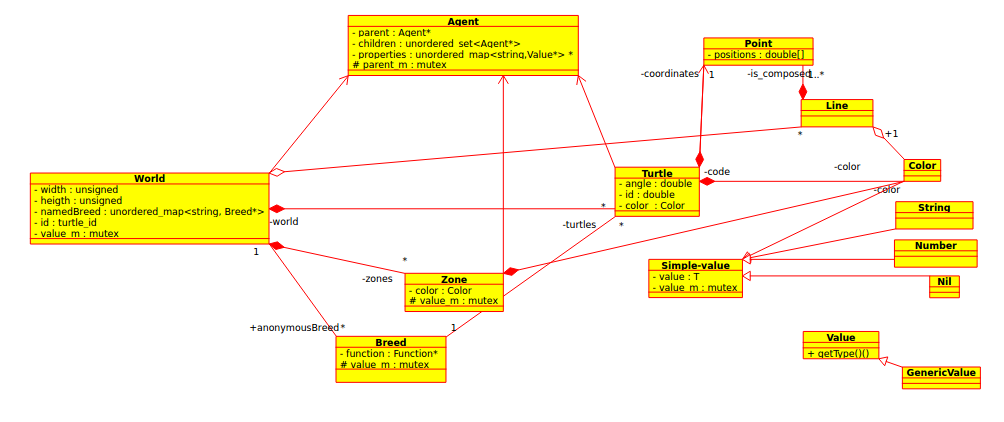
\includegraphics[scale=0.45]{doc/report/uml/v02reel.png}
\end{figure}
CAPTURE D'ECRAN DE L'APPLI
\newpage

\section{Sprint 3}

Lors du sprint 3, nous avons mis en place des pointers intelligents dans toutes nos classes REFERENCE A UN ARTICLE.\\
Nous avons ajouté des sous-classes de Function Standart-function et User-function pour représenter les fonctions standarts du langages. On les différencies des instructions par leurs parenthéses derrière leur nom.\\ Les user-function représentent les fonctions crées par l'utilisateur.\\
L'ajout de table fait aussi partit de ce sprint. Nous avons choisi, pour notre langage un seul type de conteneur : les tableaux.
Nous avons choisi de les écrire façon php, avec des accolades.\\
EXEMPLE DE CODE !!\\
Le but de ce sprint été la mise en place de la communication entre les agents. Les tortues peuvent "communiquer" avec les zones par écriture dans leurs propriétés. Les tortues peuvent communiquer entre elles grâce à des méthodes comme sendAll(message), recv(), etc...\\
Voir figure~\ref{v0.3} page~\pageref{v0.3}.
\begin{figure}[h]
\caption{\label{v0.3} UML version 0.3}
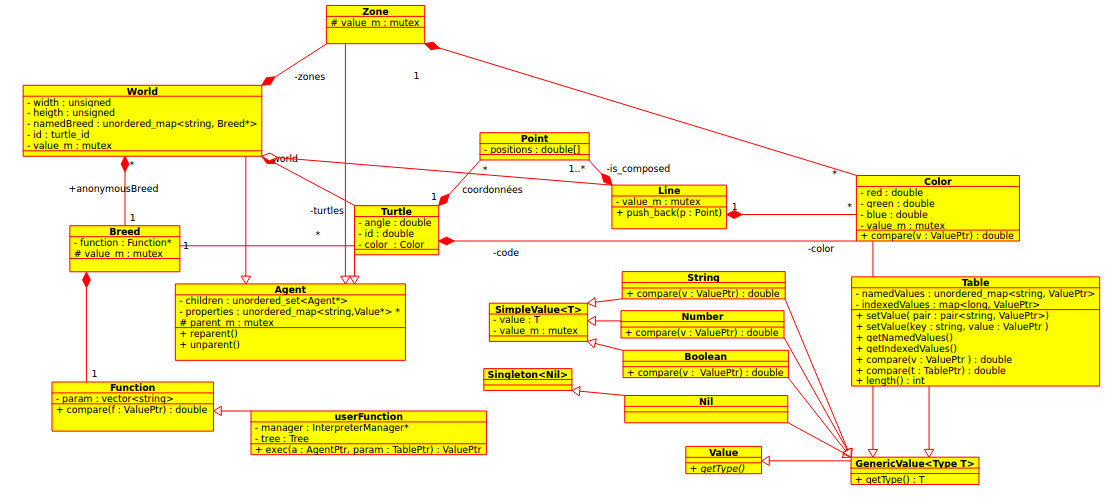
\includegraphics[scale=0.4]{doc/report/uml/v03.png}
\end{figure}
\section{Sprint 4}
Nous devons ajouter des fonctionnalités tel que la maitrise du temps et l'exportation du modèle. Ces ajouts ne provoque pas de changement du coté du modèle, si ce n'est quelques méthodes dans les classes World et Turtle et zone pour l'exportation du modèle.\\
L'exportation du modèle consiste à créer une sauvegarde de l'état du modèle à un instant t dans un fichier JSON.\\
Cela permettra ensuite, en passant par une transformation en CSV, d'avoir un tableau avec toutes ces données, ce qui permettra d'avoir des diagrammes de l'évolution du monde.\\

La maîtrise du temps se fait grâce à un bouton pause, qui arrête les threads qui s'executent, ou par un slider qui permet de ralentir ou de diminuer la vitesse. Cela se fait dans le code grâce à une méthode wait() qui fait lance sleep() sur le thread.\\

Le sprint 5 n'apporte pas de grand changement dans le modèle.

